\pdfoptionpdfminorversion=7
\documentclass[11pt]{beamer}

\mode<presentation>
{
  \usetheme{Rochester}       % or try default, Darmstadt, Warsaw, ...
  \usecolortheme{default} % or try albatross, beaver, crane, ...
  \usefonttheme{serif}    % or try default, structurebold, ...
  \setbeamertemplate{navigation symbols}{}
  \setbeamertemplate{caption}[numbered]
}

\usepackage[utf8x]{inputenc}
\usepackage{booktabs} 
\usepackage{bibentry}
\usepackage{amsmath}
\usepackage{listings}
\usepackage{graphicx}
\usepackage{lmodern}

\title{Nuevo algoritmo para detección de contacto entre poliedros}
\institute[Universidad Andrés Bello]{

\includegraphics[width=0.3\linewidth]{img/unab.png}
\hspace*{-0.5cm}~
}
\author{Yerko Zec}
\date{\today}


\begin{document}
\begin{frame}[plain]
  \titlepage
\end{frame}

\addtocounter{framenumber}{-1}

\begin{frame}{Contenido}
 \tableofcontents
\end{frame}


\section{Motivación}
\begin{frame}{Motivación}
    \begin{itemize}
     \item Detección de contacto entre poliedros.
     \item Simulación de grandes movimientos de rocas propuesto por Cundall \cite{1988-Cundall}.
     \item Nueva propuesta para detección de contacto entre poliedros.
     \item Problema de detección aun no se encuentra resuelto en su totalidad.
    \end{itemize}
\end{frame}

\section{Historia}
\begin{frame}{Historia}
 \begin{itemize}
  \item En 1971 Cundall \cite{1988-Cundall} elaboro un método llamado Discrete Element Method(DEM).
  \item DEM está dividido en 3 fases: neighbor search, contact detection y force calculations.  
  \item Esta propuesta simula grandes movimiento de partículas, los cuales son calculados mediante la implementación de distintos algoritmos.
  \item Hasta la fecha existen más de 15 algoritmos para la detección de contacto entre partículas.
 \end{itemize}
\end{frame}

\begin{frame}{Common-Plane}
 \begin{itemize}
  \item En 1988 Cundall\cite{1988-Cundall} propuso un algoritmo llamado Common-Plane (CP)
  \item Mencionando algunos algoritmos utilizados a lo largo de la historia son: CP, FCP, MR, SLM, Multi-grid y MSC entre otros.
  \item Estos algoritmos empezaron desde la misma base que ocupa el algoritmo Common-Plane.
 \end{itemize}
\end{frame}

\begin{frame}{Common-Plane}
 \begin{itemize}
  \item Common-Plane(CP), fue primeramente creado por Cundall en 1988.
  \item El principio de este algoritmo, es localizar un plano entre dos figuras e ir calculando la distancias.
  
  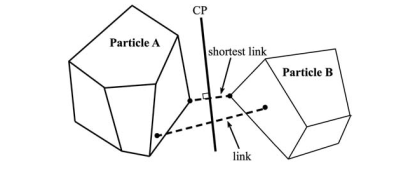
\includegraphics[width=0.5\linewidth]{img/CP}
 \end{itemize}
\end{frame}

\begin{frame}{Fast Common-Plane}
 \begin{itemize}
  \item En 2004 Nezami \cite{2004-Nezami} propuso una nueva propuesta para el calculo del CP y se llamo Fast Common-Plane (FCP).
  \item Con esta nueva propuesta mejoro el orden del algoritmo por ello la eficiencia.
  
  \includegraphics[width = 0.5\linewidth]{img/Diagrama-FCP}
 \end{itemize}
\end{frame}

\begin{frame}{Shortest Link Method}
 \begin{itemize}
  \item Nezami en 2006 \cite{2006-Nezami} propuso otro algoritmo el cual ocupa como base FCP.
  \item En base a resultados expuestos por Nezami \cite{2006-Nezami} SLM es 17 veces mas rápido que otros algoritmos convencionales.
  
  \includegraphics[width=0.5\linewidth]{img/SLM}
 \end{itemize}
\end{frame}

\begin{frame}{Multi-shell Contact Detection}
 \begin{itemize}
  \item %algoritmo MSC(multi-shell contact detection)
 \end{itemize}
\end{frame}

\section{Problema}
\begin{frame}{Problema}
\begin{itemize}
    \item Computacionalmente costoso.
    \item Eficiencia en algoritmos de detección de contacto.
\end{itemize}
\end{frame}

\section{Objetivo}
\begin{frame}{Objetivo}
\begin{block}{Objetivo General}
 \begin{itemize}
    \item Detectar de forma eficiente y eficaz el contacto entre poliedros.
 \end{itemize}
\end{block}
\begin{block}{Objetivo Especifico}
 \begin{itemize}
  \item 
 \end{itemize}
\end{block}
\end{frame}     

\section{Hipótesis}
\begin{frame}{Hipótesis}
\begin{itemize}
    \item Entregar nuevo propuesta para la detección de contacto
\end{itemize}
\end{frame}

\section{Metodología}
\begin{frame}{Metodología}
\begin{itemize}
    \item Entregar nueva propuesta para la detección de contacto
\end{itemize}
\end{frame}

\medskip
\bibliographystyle{plain}
\bibliography{/home/yerkozec/Desktop/pt/memoria/Referencia}

\end{document}
